% ========================================================
% PROJECT TEMPLATE, *KNOWLEDGE DISCOVERY*, Summer 2018
% University of Potsdam, by Christoph Schommer, University
% of Luxembourg; 
% ========================================================

\documentclass[11pt]{article}
\usepackage{geometry}
\usepackage{enumitem}
\usepackage{graphicx}
\usepackage[usenames,dvipsnames]{color}
\usepackage{hyperref}

%
\newcommand{\code}[1]{\textbf{#1}}
\newcommand{\para}[0]{\par\vspace{0.5cm}}

%
\def\MakeMeBlue#1{\textcolor{Blue}{#1}}
\pagenumbering{arabic}
%

\parindent 0pt

%

\title{\MakeMeBlue{Overview of measures of similarity between random variables in a sample}}
\author{Miroslav Vitkov}
\date{\today}

% ========================================================
\begin{document}
\maketitle

% ========================================================
\section{Introduction}
This report explores the following measures over a pair of random variable:
\begin{itemize}
    \item{Pearson correlation coefficient}
    \item{Spearman correlation coefficient}
    \item{Kendall correlation coefficient\cite{q3}}
    \item{Kullback–Leibler divergence}
    \item{Euclidean distance.}
\end{itemize}
\para
Explored are pairs of features in the `Household Power Consumption database` and are plotted.

% ========================================================
\section{Related Work}
Croux et al\cite{q4} demonstrate that a two variable Spearman or Kendall correlation measure is resistant to outliers.
\para
Chujai et al\cite{q1} use the same dataset to train an ARIMA regression algorithm.
They fail to mention the misleading dataset precision, addressed later in this work.

% ========================================================
\section{Methodology}
\subsection{Code}
\code{R} with \code{tidyverse} has been used as modern\cite{q5} statistical software.
The source code is available at \url{https://github.com/MiroslavVitkov/cogsys/tree/master/mine}

\subsection{Pearson correlation coefficient}
This is the widely used 'regression coefficient'\cite{q8} applied to a sample:
$$ r_{xy} = \frac{\sum(x_i - \overline{x})(y_i - \overline{y})}
                 {\sqrt{\sum(x_i - \overline{x})^2*\sum(y_i - \overline{y})^2}} $$
\begin{figure}[!htp]
  \centering
    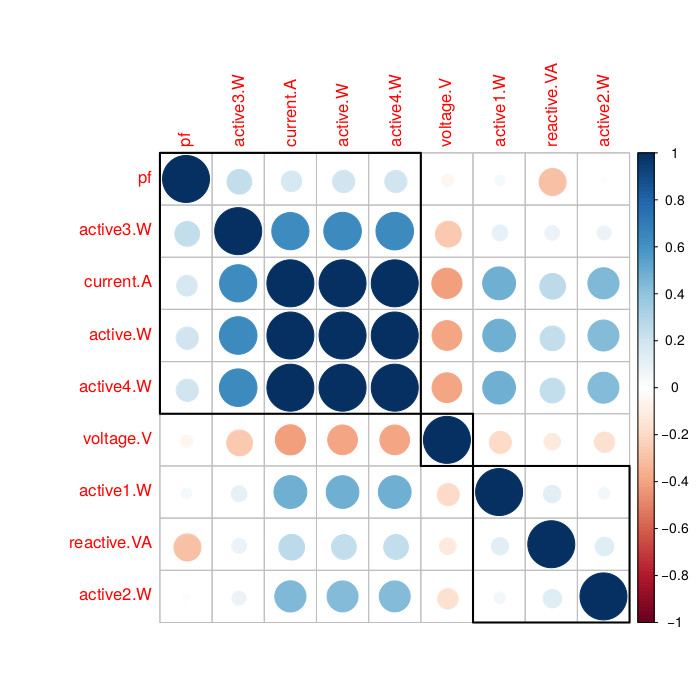
\includegraphics[width=0.8\textwidth]{img/pearson}
    \caption{Pearson cross-correlation of the dataset.}
\end{figure}

\subsection{Spearman correlation coefficient}
The Spearman correlation is defined as the Pearson correlation among the ranks of the points.
Being a ranked correlation, it: 
\begin{itemize}
    \item{Can represent non-linear dependencies, as long as they are monotonic.\cite{q9}}
    \item{Is less sensitive to strong outliers than Pearson correlation\cite{q4}\cite{q9}.}
\end{itemize}

\begin{figure}[!htp]
  \centering
    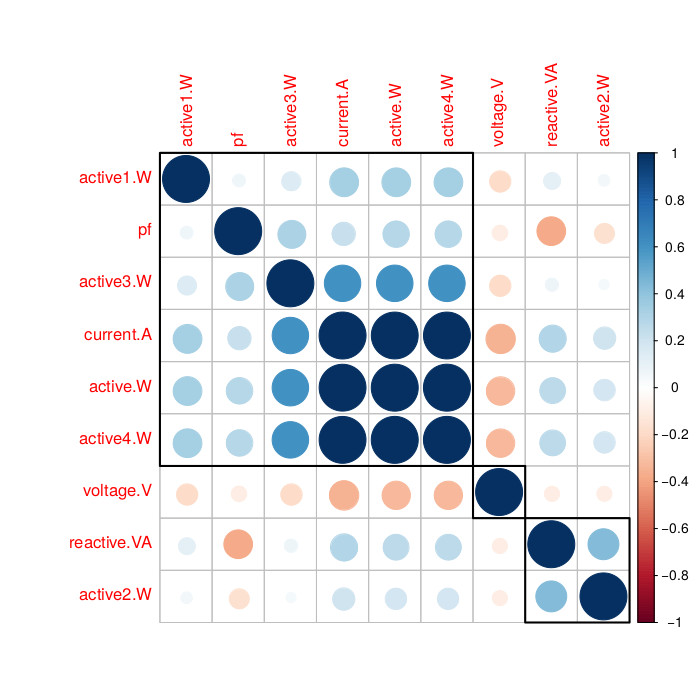
\includegraphics[width=0.8\textwidth]{img/spearman}
    \caption{Spearman rank of the dataset}
\end{figure}

\subsection{Kendall correlation coefficient}
This is another rank correlation, expressed by\cite{q10}:
$$ \tau = \frac{({number of concordant points}-{number of discordant points})}
                 {n(n-1)/2} $$
\para
This method turned out to be significantly slower than any of the other 4.
Consequently, here is presented a diagram of only a small part of the dataset.
The sampling is performed without randomisation.

\begin{figure}[!htp]
  \centering
    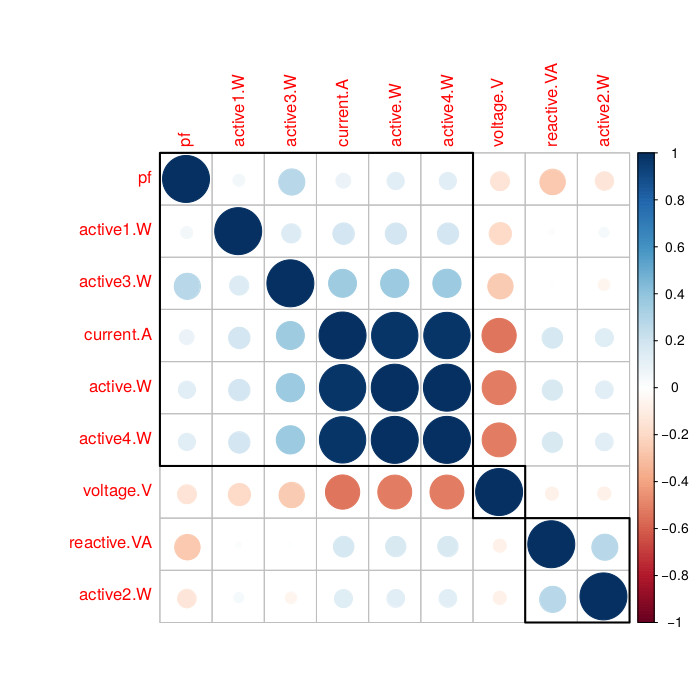
\includegraphics[width=0.8\textwidth]{img/kendall}
    \caption{Kendall rank correlation over the first 10 000 points}
\end{figure}

\subsection{Proximity}
The previous 3 scores have range [-1, 1] with 0 meaning "largest dissimilarity".
The next 2 estimators are a pseudo-distance and a distance.
Thus their range is [0, inf) with 0 meaning "smallest dissimilarity".
\para
In order to arrive at comparable measures, a function \code{f()} needs to be designed.
\code{f} should map the latter interval into the first.
Thus all five measures will be comparable and plotable by the same tools.
\para
The requirements for such a function would be:
\begin{enumerate}
    \item{monotonic - if $x1 \ge x2$ then $f(x1) \ge f(x2)$}
    \item{work on a discrete sample}
\end{enumerate}
\para
The chosen solution for this project is a chain of simple functions:
$$ f(x) = scale(trans(log(clamp(x^{-1})))) $$
, where \\
$ clamp() $ - replace \code{Inf} with a large number; is first trained on the data  \\
$ trans() $ - translate a matrix with the minimum amount, which results in all entries being positive  \\  
$ norm(x_i) = x_i/\sum_i x_i $  \\

\subsection{Kullback–Leibler divergence}
KL is a measure of dissimilarity between distributions.
It's discrete form can be expressed as
$$ D_{KL}(p, q) = \sum p_i \log\frac{p_i}{q_i} $$
\para
The Kullback–Leibler divergence is defined only if for all i, Q(i) = 0 implies P(i) = 0 (absolute continuity).\cite{q11}
For this reason, the current implementation smooths the Q distribution with a weak uniform prior.
\begin{figure}[!htp]
  \centering
    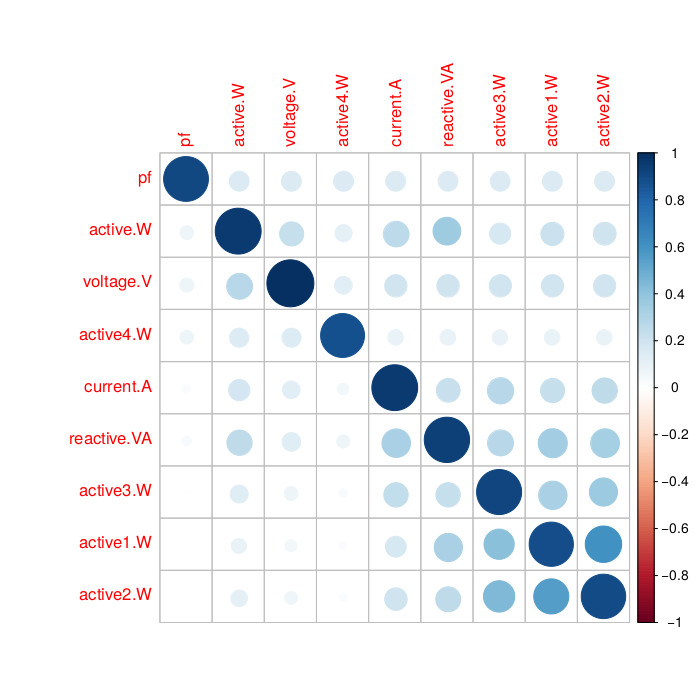
\includegraphics[width=0.8\textwidth]{img/kl}
    \caption{f(Kullback–Leibler divergence)}
\end{figure}
\para

\subsection{Euclidean distance}

\begin{figure}[!htp]
  \centering
    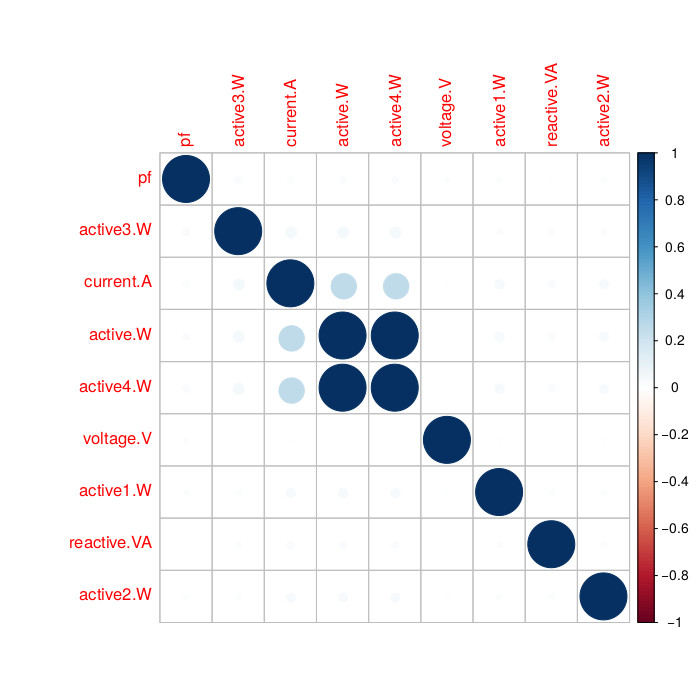
\includegraphics[width=0.8\textwidth]{img/euclid}
    \caption{f(Euclidean distance)}
\end{figure}
\para

% ========================================================
\section{Implementation}
\subsection{Getting the data}
The database is of significant size, spanning 2075259 instances.
This is time consuming both for a human and for a CPU to work on.
Therefore, the script \code{get\_dataset.sh} has been written.
It accepts a numeric parameter of how many instances to be downloaded.
If no parameter is passed, the whole dataset is downloaded.

\subsection{Reading the data}
The dataset is read in, converted to floating point numbers, then converted to SI units.

\subsection{Sanity checking}
At this point it becomes evident the dataset claims higher precision than demonstrated.
Consider the 26-th sample: \code{16/12/2006;17:49:00;3.248;0.000;236.660;13.600;0.000;0.000;17.000}
Power factor is defined\cite{q6} as follows:
$$ {pf} = \frac{P}{S} $$
,where:  
P, [W] - real power  
S, [VA] - apparent power  

Plugging the numbers in:
$$ {pf} = P / (U * I) = $$
$$ 3.248kW / 236.660V * 13.600A = $$
$$ 1.00914 $$

And ${pf}$ is defined on the interval [-1, 1]\cite{q6}.
\para
As is well known,  "Trailing zeros to the right of the decimal ARE significant"\cite{q7}.
In the above example, there are 3 digits of accuracy, which are fixed at 0.
Had those zeroes not been written, the dataset would have claimed less precision.
Now, however, it is inaccurate and thus internally inconsistent.

\subsection{Cleaning the data}
1.251844\% Of the input data has been dropped because it is missing or an outlier.
52\% of the database would be dropped if ${pf}$ range is checked, and it thus not done.

% ========================================================
\section{Conclusion}
It was noticed that the used dataset claims higher precision that it actually provides.
\para
All plots show the obvious interconnection between \code{active4.W, active.W, current.A}.
However the Kullback–Leibler divergence makes different and vague predictions.
\para
Further work should involve auto-correlations and time-shifted cross-correlations and dependencies.
Kullback–Leibler divergence with previously median-aligned distributions and with various smoothing
% ========================================================

\begin{thebibliography}{9}

\bibitem{q1}
  Pasapitch Chujai, Nittaya Kerdprasop, and Kittisak Kerdprasop,
  \textit{Time Series Analysis of Household Electric Consumption with ARIMA and ARMA Models},
  Proceedings of the International MultiConference of Engineers and Computer Scientists 2013 Vol I,
  IMECS 2013, March 13 - 15, 2013, Hong Kong

\bibitem{q2}
  Georges Hébrail,
  \textit{P RIVACY - PRESERVING USE OF INDIVIDUAL SMART METERING DATA FOR CUSTOMER SERVICES}

\bibitem{q3}
    Kendall, M. G. (1938).
    \textit{A new measure of rank correlation, Biometrika}, *30*, 81-93.
    doi: 10.1093/biomet/30.1-2.81
    (URL: \url{http://doi.org/10.1093/biomet/30.1-2.81})

\bibitem{q4}
    Christophe Croux · Catherine Dehon
    Influence functions of the Spearman and Kendall correlation measures

\bibitem{q5}
    Hadley Wickham
    tidyverse 1.0.0
    \url{https://blog.rstudio.com/2016/09/15/tidyverse-1-0-0/}

\bibitem{q6}
    Trial-Use Standard Definitions for the Measurement of Electric Power Quantities Under Sinusoidal, Nonsinusoidal, Balanced, or Unbalanced Conditions, IEEE, 2000, ISBN 0-7381-1963-6, Std. 1459-2000. Note 1, section 3.1.1.1, when defining the quantities for power factor, asserts that real power only flows to the load and can never be negative. As of 2013, one of the authors acknowledged that this note was incorrect, and is being revised for the next edition. See \url{http://powerstandards.com/Shymanski/draft.pdf}

\bibitem{q7}
    \url{http://ccnmtl.columbia.edu/projects/mmt/frontiers/web/chapter_5/6665.html}

\bibitem{q8}
Rodgers, J. L.; Nicewander, W. A. (1988). "Thirteen ways to look at the correlation coefficient". The American Statistician. 42 (1): 59–66. doi:10.1080/00031305.1988.10475524. JSTOR 2685263.

\bibitem{q9}
 Lehman, Ann (2005).
 Jmp For Basic Univariate And Multivariate Statistics: A Step-by-step Guide. Cary, NC: SAS Press. p. 123. ISBN 1-59047-576-3.

\bibitem{q10}
 Nelsen, R.B. (2001) [1994], "Kendall tau metric", in Hazewinkel, Michiel, Encyclopedia of Mathematics, Springer Science+Business Media B.V. / Kluwer Academic Publishers, ISBN 978-1-55608-010-4

\bibitem{q11}
 MacKay, David J.C. (2003). Information Theory, Inference, and Learning Algorithms (First ed.). Cambridge University Press. p. 34. 

\end{thebibliography}

\end{document}

